% Options for packages loaded elsewhere
% Options for packages loaded elsewhere
\PassOptionsToPackage{unicode}{hyperref}
\PassOptionsToPackage{hyphens}{url}
\PassOptionsToPackage{dvipsnames,svgnames,x11names}{xcolor}
%
\documentclass[
  letterpaper,
  DIV=11,
  numbers=noendperiod]{scrartcl}
\usepackage{xcolor}
\usepackage{amsmath,amssymb}
\setcounter{secnumdepth}{-\maxdimen} % remove section numbering
\usepackage{iftex}
\ifPDFTeX
  \usepackage[T1]{fontenc}
  \usepackage[utf8]{inputenc}
  \usepackage{textcomp} % provide euro and other symbols
\else % if luatex or xetex
  \usepackage{unicode-math} % this also loads fontspec
  \defaultfontfeatures{Scale=MatchLowercase}
  \defaultfontfeatures[\rmfamily]{Ligatures=TeX,Scale=1}
\fi
\usepackage{lmodern}
\ifPDFTeX\else
  % xetex/luatex font selection
\fi
% Use upquote if available, for straight quotes in verbatim environments
\IfFileExists{upquote.sty}{\usepackage{upquote}}{}
\IfFileExists{microtype.sty}{% use microtype if available
  \usepackage[]{microtype}
  \UseMicrotypeSet[protrusion]{basicmath} % disable protrusion for tt fonts
}{}
\makeatletter
\@ifundefined{KOMAClassName}{% if non-KOMA class
  \IfFileExists{parskip.sty}{%
    \usepackage{parskip}
  }{% else
    \setlength{\parindent}{0pt}
    \setlength{\parskip}{6pt plus 2pt minus 1pt}}
}{% if KOMA class
  \KOMAoptions{parskip=half}}
\makeatother
% Make \paragraph and \subparagraph free-standing
\makeatletter
\ifx\paragraph\undefined\else
  \let\oldparagraph\paragraph
  \renewcommand{\paragraph}{
    \@ifstar
      \xxxParagraphStar
      \xxxParagraphNoStar
  }
  \newcommand{\xxxParagraphStar}[1]{\oldparagraph*{#1}\mbox{}}
  \newcommand{\xxxParagraphNoStar}[1]{\oldparagraph{#1}\mbox{}}
\fi
\ifx\subparagraph\undefined\else
  \let\oldsubparagraph\subparagraph
  \renewcommand{\subparagraph}{
    \@ifstar
      \xxxSubParagraphStar
      \xxxSubParagraphNoStar
  }
  \newcommand{\xxxSubParagraphStar}[1]{\oldsubparagraph*{#1}\mbox{}}
  \newcommand{\xxxSubParagraphNoStar}[1]{\oldsubparagraph{#1}\mbox{}}
\fi
\makeatother

\usepackage{color}
\usepackage{fancyvrb}
\newcommand{\VerbBar}{|}
\newcommand{\VERB}{\Verb[commandchars=\\\{\}]}
\DefineVerbatimEnvironment{Highlighting}{Verbatim}{commandchars=\\\{\}}
% Add ',fontsize=\small' for more characters per line
\usepackage{framed}
\definecolor{shadecolor}{RGB}{241,243,245}
\newenvironment{Shaded}{\begin{snugshade}}{\end{snugshade}}
\newcommand{\AlertTok}[1]{\textcolor[rgb]{0.68,0.00,0.00}{#1}}
\newcommand{\AnnotationTok}[1]{\textcolor[rgb]{0.37,0.37,0.37}{#1}}
\newcommand{\AttributeTok}[1]{\textcolor[rgb]{0.40,0.45,0.13}{#1}}
\newcommand{\BaseNTok}[1]{\textcolor[rgb]{0.68,0.00,0.00}{#1}}
\newcommand{\BuiltInTok}[1]{\textcolor[rgb]{0.00,0.23,0.31}{#1}}
\newcommand{\CharTok}[1]{\textcolor[rgb]{0.13,0.47,0.30}{#1}}
\newcommand{\CommentTok}[1]{\textcolor[rgb]{0.37,0.37,0.37}{#1}}
\newcommand{\CommentVarTok}[1]{\textcolor[rgb]{0.37,0.37,0.37}{\textit{#1}}}
\newcommand{\ConstantTok}[1]{\textcolor[rgb]{0.56,0.35,0.01}{#1}}
\newcommand{\ControlFlowTok}[1]{\textcolor[rgb]{0.00,0.23,0.31}{\textbf{#1}}}
\newcommand{\DataTypeTok}[1]{\textcolor[rgb]{0.68,0.00,0.00}{#1}}
\newcommand{\DecValTok}[1]{\textcolor[rgb]{0.68,0.00,0.00}{#1}}
\newcommand{\DocumentationTok}[1]{\textcolor[rgb]{0.37,0.37,0.37}{\textit{#1}}}
\newcommand{\ErrorTok}[1]{\textcolor[rgb]{0.68,0.00,0.00}{#1}}
\newcommand{\ExtensionTok}[1]{\textcolor[rgb]{0.00,0.23,0.31}{#1}}
\newcommand{\FloatTok}[1]{\textcolor[rgb]{0.68,0.00,0.00}{#1}}
\newcommand{\FunctionTok}[1]{\textcolor[rgb]{0.28,0.35,0.67}{#1}}
\newcommand{\ImportTok}[1]{\textcolor[rgb]{0.00,0.46,0.62}{#1}}
\newcommand{\InformationTok}[1]{\textcolor[rgb]{0.37,0.37,0.37}{#1}}
\newcommand{\KeywordTok}[1]{\textcolor[rgb]{0.00,0.23,0.31}{\textbf{#1}}}
\newcommand{\NormalTok}[1]{\textcolor[rgb]{0.00,0.23,0.31}{#1}}
\newcommand{\OperatorTok}[1]{\textcolor[rgb]{0.37,0.37,0.37}{#1}}
\newcommand{\OtherTok}[1]{\textcolor[rgb]{0.00,0.23,0.31}{#1}}
\newcommand{\PreprocessorTok}[1]{\textcolor[rgb]{0.68,0.00,0.00}{#1}}
\newcommand{\RegionMarkerTok}[1]{\textcolor[rgb]{0.00,0.23,0.31}{#1}}
\newcommand{\SpecialCharTok}[1]{\textcolor[rgb]{0.37,0.37,0.37}{#1}}
\newcommand{\SpecialStringTok}[1]{\textcolor[rgb]{0.13,0.47,0.30}{#1}}
\newcommand{\StringTok}[1]{\textcolor[rgb]{0.13,0.47,0.30}{#1}}
\newcommand{\VariableTok}[1]{\textcolor[rgb]{0.07,0.07,0.07}{#1}}
\newcommand{\VerbatimStringTok}[1]{\textcolor[rgb]{0.13,0.47,0.30}{#1}}
\newcommand{\WarningTok}[1]{\textcolor[rgb]{0.37,0.37,0.37}{\textit{#1}}}

\usepackage{longtable,booktabs,array}
\usepackage{calc} % for calculating minipage widths
% Correct order of tables after \paragraph or \subparagraph
\usepackage{etoolbox}
\makeatletter
\patchcmd\longtable{\par}{\if@noskipsec\mbox{}\fi\par}{}{}
\makeatother
% Allow footnotes in longtable head/foot
\IfFileExists{footnotehyper.sty}{\usepackage{footnotehyper}}{\usepackage{footnote}}
\makesavenoteenv{longtable}
\usepackage{graphicx}
\makeatletter
\newsavebox\pandoc@box
\newcommand*\pandocbounded[1]{% scales image to fit in text height/width
  \sbox\pandoc@box{#1}%
  \Gscale@div\@tempa{\textheight}{\dimexpr\ht\pandoc@box+\dp\pandoc@box\relax}%
  \Gscale@div\@tempb{\linewidth}{\wd\pandoc@box}%
  \ifdim\@tempb\p@<\@tempa\p@\let\@tempa\@tempb\fi% select the smaller of both
  \ifdim\@tempa\p@<\p@\scalebox{\@tempa}{\usebox\pandoc@box}%
  \else\usebox{\pandoc@box}%
  \fi%
}
% Set default figure placement to htbp
\def\fps@figure{htbp}
\makeatother





\setlength{\emergencystretch}{3em} % prevent overfull lines

\providecommand{\tightlist}{%
  \setlength{\itemsep}{0pt}\setlength{\parskip}{0pt}}



 


\KOMAoption{captions}{tableheading}
\makeatletter
\@ifpackageloaded{caption}{}{\usepackage{caption}}
\AtBeginDocument{%
\ifdefined\contentsname
  \renewcommand*\contentsname{Table of contents}
\else
  \newcommand\contentsname{Table of contents}
\fi
\ifdefined\listfigurename
  \renewcommand*\listfigurename{List of Figures}
\else
  \newcommand\listfigurename{List of Figures}
\fi
\ifdefined\listtablename
  \renewcommand*\listtablename{List of Tables}
\else
  \newcommand\listtablename{List of Tables}
\fi
\ifdefined\figurename
  \renewcommand*\figurename{Figure}
\else
  \newcommand\figurename{Figure}
\fi
\ifdefined\tablename
  \renewcommand*\tablename{Table}
\else
  \newcommand\tablename{Table}
\fi
}
\@ifpackageloaded{float}{}{\usepackage{float}}
\floatstyle{ruled}
\@ifundefined{c@chapter}{\newfloat{codelisting}{h}{lop}}{\newfloat{codelisting}{h}{lop}[chapter]}
\floatname{codelisting}{Listing}
\newcommand*\listoflistings{\listof{codelisting}{List of Listings}}
\makeatother
\makeatletter
\makeatother
\makeatletter
\@ifpackageloaded{caption}{}{\usepackage{caption}}
\@ifpackageloaded{subcaption}{}{\usepackage{subcaption}}
\makeatother
\usepackage{bookmark}
\IfFileExists{xurl.sty}{\usepackage{xurl}}{} % add URL line breaks if available
\urlstyle{same}
\hypersetup{
  pdftitle={EV Power - Lab 4 Project Report},
  colorlinks=true,
  linkcolor={blue},
  filecolor={Maroon},
  citecolor={Blue},
  urlcolor={Blue},
  pdfcreator={LaTeX via pandoc}}


\title{EV Power - Lab 4 Project Report}
\author{}
\date{}
\begin{document}
\maketitle


\section{Example Solution 1}\label{example-solution-1}

\subsection{\texorpdfstring{\textbf{Part 0:
libraries}}{Part 0: libraries}}\label{part-0-libraries}

\begin{Shaded}
\begin{Highlighting}[]
\FunctionTok{library}\NormalTok{(readr)}
\FunctionTok{library}\NormalTok{(dplyr)}
\end{Highlighting}
\end{Shaded}

\begin{verbatim}

Attaching package: 'dplyr'
\end{verbatim}

\begin{verbatim}
The following objects are masked from 'package:stats':

    filter, lag
\end{verbatim}

\begin{verbatim}
The following objects are masked from 'package:base':

    intersect, setdiff, setequal, union
\end{verbatim}

\begin{Shaded}
\begin{Highlighting}[]
\FunctionTok{library}\NormalTok{(tidyr)}
\FunctionTok{library}\NormalTok{(stringr)}
\FunctionTok{library}\NormalTok{(tibble)}
\end{Highlighting}
\end{Shaded}

\subsection{\texorpdfstring{\textbf{Part 1:} \textbf{Defining Research
Question}}{Part 1: Defining Research Question}}\label{part-1-defining-research-question}

Chosen Question: Which states in 2023 get a higher share of their total
energy from renewable sources?

\subsection{\texorpdfstring{\textbf{Part 2: Data Preparation and
Cleaning}}{Part 2: Data Preparation and Cleaning}}\label{part-2-data-preparation-and-cleaning}

\begin{Shaded}
\begin{Highlighting}[]
\DocumentationTok{\#\# Part 1: helper to standardize column names}

\NormalTok{clean\_names }\OtherTok{\textless{}{-}} \ControlFlowTok{function}\NormalTok{(df) \{}
\NormalTok{  new\_names }\OtherTok{\textless{}{-}} \FunctionTok{names}\NormalTok{(df) }\SpecialCharTok{|\textgreater{}}
    \FunctionTok{str\_trim}\NormalTok{() }\SpecialCharTok{|\textgreater{}}
    \FunctionTok{str\_replace\_all}\NormalTok{(}\StringTok{"[\^{}A{-}Za{-}z0{-}9]+"}\NormalTok{, }\StringTok{"\_"}\NormalTok{) }\SpecialCharTok{|\textgreater{}}
    \FunctionTok{tolower}\NormalTok{() }\SpecialCharTok{|\textgreater{}}
    \FunctionTok{str\_replace\_all}\NormalTok{(}\StringTok{"\^{}\_|\_$"}\NormalTok{, }\StringTok{""}\NormalTok{)}
  \FunctionTok{names}\NormalTok{(df) }\OtherTok{\textless{}{-}}\NormalTok{ new\_names}
\NormalTok{  df}
\NormalTok{\}}

\NormalTok{renew\_2023 }\OtherTok{\textless{}{-}} \FunctionTok{read\_csv}\NormalTok{(}\StringTok{"data/renew{-}use{-}2023.csv"}\NormalTok{) }\SpecialCharTok{|\textgreater{}} \FunctionTok{clean\_names}\NormalTok{()}
\end{Highlighting}
\end{Shaded}

\begin{verbatim}
Rows: 260 Columns: 3
-- Column specification --------------------------------------------------------
Delimiter: ","
chr (3): State, Energy_Source, Renewable_Use_2023

i Use `spec()` to retrieve the full column specification for this data.
i Specify the column types or set `show_col_types = FALSE` to quiet this message.
\end{verbatim}

\begin{Shaded}
\begin{Highlighting}[]
\NormalTok{total\_2023 }\OtherTok{\textless{}{-}} \FunctionTok{read\_csv}\NormalTok{(}\StringTok{"data/total{-}use{-}2023.csv"}\NormalTok{) }\SpecialCharTok{|\textgreater{}} \FunctionTok{clean\_names}\NormalTok{()}
\end{Highlighting}
\end{Shaded}

\begin{verbatim}
Rows: 5 Columns: 53
-- Column specification --------------------------------------------------------
Delimiter: ","
chr  (1): Energy_Source
dbl (52): AK, AL, AR, AZ, CA, CO, CT, DC, DE, FL, GA, HI, IA, ID, IL, IN, KS...

i Use `spec()` to retrieve the full column specification for this data.
i Specify the column types or set `show_col_types = FALSE` to quiet this message.
\end{verbatim}

\begin{Shaded}
\begin{Highlighting}[]
\NormalTok{ev\_raw     }\OtherTok{\textless{}{-}} \FunctionTok{read\_csv}\NormalTok{(}\StringTok{"data/ev{-}registrations{-}by{-}state{-}2023.csv"}\NormalTok{) }\SpecialCharTok{|\textgreater{}} \FunctionTok{clean\_names}\NormalTok{()}
\end{Highlighting}
\end{Shaded}

\begin{verbatim}
New names:
Rows: 54 Columns: 2
-- Column specification
-------------------------------------------------------- Delimiter: "," chr
(2): electric vehicle registrations_by_state (2023), ...2
i Use `spec()` to retrieve the full column specification for this data. i
Specify the column types or set `show_col_types = FALSE` to quiet this message.
* `` -> `...2`
\end{verbatim}

\begin{Shaded}
\begin{Highlighting}[]
\NormalTok{renew\_2023\_clean }\OtherTok{\textless{}{-}}
\NormalTok{  renew\_2023 }\SpecialCharTok{|\textgreater{}}
  \FunctionTok{mutate}\NormalTok{(}
    \AttributeTok{state =} \FunctionTok{toupper}\NormalTok{(state),}
    \AttributeTok{renewable\_use\_2023\_num =} \FunctionTok{as.numeric}\NormalTok{(}
      \FunctionTok{na\_if}\NormalTok{(}
        \FunctionTok{str\_replace\_all}\NormalTok{(}
          \FunctionTok{as.character}\NormalTok{(renewable\_use\_2023),}
          \StringTok{"[\^{}0{-}9.]"}\NormalTok{,}
          \StringTok{""}
\NormalTok{        ),}
        \StringTok{""}
\NormalTok{      )}
\NormalTok{    )}
\NormalTok{  )}

\NormalTok{renew\_by\_state\_2023 }\OtherTok{\textless{}{-}}
\NormalTok{  renew\_2023\_clean }\SpecialCharTok{|\textgreater{}}
  \FunctionTok{group\_by}\NormalTok{(state) }\SpecialCharTok{|\textgreater{}}
  \FunctionTok{summarize}\NormalTok{(}
    \AttributeTok{renewable\_total\_2023 =} \FunctionTok{sum}\NormalTok{(renewable\_use\_2023\_num, }\AttributeTok{na.rm =} \ConstantTok{TRUE}\NormalTok{),}
    \AttributeTok{.groups =} \StringTok{"drop"}
\NormalTok{  )}

\NormalTok{total\_2023\_long }\OtherTok{\textless{}{-}}
\NormalTok{  total\_2023 }\SpecialCharTok{|\textgreater{}}
  \FunctionTok{pivot\_longer}\NormalTok{(}
    \AttributeTok{cols =} \SpecialCharTok{{-}}\NormalTok{energy\_source,}
    \AttributeTok{names\_to =} \StringTok{"state"}\NormalTok{,}
    \AttributeTok{values\_to =} \StringTok{"energy\_use\_2023"}
\NormalTok{  ) }\SpecialCharTok{|\textgreater{}}
  \FunctionTok{mutate}\NormalTok{(}
    \AttributeTok{state =} \FunctionTok{toupper}\NormalTok{(state)}
\NormalTok{  )}

\NormalTok{total\_energy\_by\_state\_2023 }\OtherTok{\textless{}{-}}
\NormalTok{  total\_2023\_long }\SpecialCharTok{|\textgreater{}}
  \FunctionTok{group\_by}\NormalTok{(state) }\SpecialCharTok{|\textgreater{}}
  \FunctionTok{summarize}\NormalTok{(}
    \AttributeTok{total\_energy\_2023 =} \FunctionTok{sum}\NormalTok{(energy\_use\_2023, }\AttributeTok{na.rm =} \ConstantTok{TRUE}\NormalTok{),}
    \AttributeTok{.groups =} \StringTok{"drop"}
\NormalTok{  )}


\NormalTok{ev\_tidy }\OtherTok{\textless{}{-}}
\NormalTok{  ev\_raw }\SpecialCharTok{|\textgreater{}}
  \FunctionTok{slice}\NormalTok{(}\SpecialCharTok{{-}}\NormalTok{(}\DecValTok{1}\SpecialCharTok{:}\DecValTok{2}\NormalTok{)) }\SpecialCharTok{|\textgreater{}}
  \FunctionTok{select}\NormalTok{(}\DecValTok{1}\NormalTok{, }\DecValTok{2}\NormalTok{) }\SpecialCharTok{|\textgreater{}}
  \FunctionTok{rename}\NormalTok{(}
    \AttributeTok{state\_full =} \DecValTok{1}\NormalTok{,}
    \AttributeTok{ev\_reg\_raw =} \DecValTok{2}
\NormalTok{  ) }\SpecialCharTok{|\textgreater{}}
  \FunctionTok{mutate}\NormalTok{(}
    \AttributeTok{state\_full =} \FunctionTok{str\_trim}\NormalTok{(state\_full),}
    \AttributeTok{ev\_registrations\_2023 =} \FunctionTok{as.numeric}\NormalTok{(}
      \FunctionTok{na\_if}\NormalTok{(}
        \FunctionTok{str\_replace\_all}\NormalTok{(}
          \FunctionTok{as.character}\NormalTok{(ev\_reg\_raw),}
          \StringTok{"[\^{}0{-}9]"}\NormalTok{,}
          \StringTok{""}
\NormalTok{        ),}
        \StringTok{""}
\NormalTok{      )}
\NormalTok{    )}
\NormalTok{  )}

\NormalTok{state\_lookup }\OtherTok{\textless{}{-}} \FunctionTok{tibble}\NormalTok{(}
  \AttributeTok{state\_full =} \FunctionTok{c}\NormalTok{(}
    \StringTok{"Alabama"}\NormalTok{,}\StringTok{"Alaska"}\NormalTok{,}\StringTok{"Arizona"}\NormalTok{,}\StringTok{"Arkansas"}\NormalTok{,}\StringTok{"California"}\NormalTok{,}\StringTok{"Colorado"}\NormalTok{,}\StringTok{"Connecticut"}\NormalTok{,}
    \StringTok{"Delaware"}\NormalTok{,}\StringTok{"District of Columbia"}\NormalTok{,}\StringTok{"Florida"}\NormalTok{,}\StringTok{"Georgia"}\NormalTok{,}\StringTok{"Hawaii"}\NormalTok{,}\StringTok{"Idaho"}\NormalTok{,}\StringTok{"Illinois"}\NormalTok{,}
    \StringTok{"Indiana"}\NormalTok{,}\StringTok{"Iowa"}\NormalTok{,}\StringTok{"Kansas"}\NormalTok{,}\StringTok{"Kentucky"}\NormalTok{,}\StringTok{"Louisiana"}\NormalTok{,}\StringTok{"Maine"}\NormalTok{,}\StringTok{"Maryland"}\NormalTok{,}\StringTok{"Massachusetts"}\NormalTok{,}
    \StringTok{"Michigan"}\NormalTok{,}\StringTok{"Minnesota"}\NormalTok{,}\StringTok{"Mississippi"}\NormalTok{,}\StringTok{"Missouri"}\NormalTok{,}\StringTok{"Montana"}\NormalTok{,}\StringTok{"Nebraska"}\NormalTok{,}\StringTok{"Nevada"}\NormalTok{,}
    \StringTok{"New Hampshire"}\NormalTok{,}\StringTok{"New Jersey"}\NormalTok{,}\StringTok{"New Mexico"}\NormalTok{,}\StringTok{"New York"}\NormalTok{,}\StringTok{"North Carolina"}\NormalTok{,}
    \StringTok{"North Dakota"}\NormalTok{,}\StringTok{"Ohio"}\NormalTok{,}\StringTok{"Oklahoma"}\NormalTok{,}\StringTok{"Oregon"}\NormalTok{,}\StringTok{"Pennsylvania"}\NormalTok{,}\StringTok{"Rhode Island"}\NormalTok{,}
    \StringTok{"South Carolina"}\NormalTok{,}\StringTok{"South Dakota"}\NormalTok{,}\StringTok{"Tennessee"}\NormalTok{,}\StringTok{"Texas"}\NormalTok{,}\StringTok{"Utah"}\NormalTok{,}\StringTok{"Vermont"}\NormalTok{,}\StringTok{"Virginia"}\NormalTok{,}
    \StringTok{"Washington"}\NormalTok{,}\StringTok{"West Virginia"}\NormalTok{,}\StringTok{"Wisconsin"}\NormalTok{,}\StringTok{"Wyoming"}\NormalTok{,}\StringTok{"Total"}
\NormalTok{  ),}
  \AttributeTok{state =} \FunctionTok{c}\NormalTok{(}
    \StringTok{"AL"}\NormalTok{,}\StringTok{"AK"}\NormalTok{,}\StringTok{"AZ"}\NormalTok{,}\StringTok{"AR"}\NormalTok{,}\StringTok{"CA"}\NormalTok{,}\StringTok{"CO"}\NormalTok{,}\StringTok{"CT"}\NormalTok{,}
    \StringTok{"DE"}\NormalTok{,}\StringTok{"DC"}\NormalTok{,}\StringTok{"FL"}\NormalTok{,}\StringTok{"GA"}\NormalTok{,}\StringTok{"HI"}\NormalTok{,}\StringTok{"ID"}\NormalTok{,}\StringTok{"IL"}\NormalTok{,}
    \StringTok{"IN"}\NormalTok{,}\StringTok{"IA"}\NormalTok{,}\StringTok{"KS"}\NormalTok{,}\StringTok{"KY"}\NormalTok{,}\StringTok{"LA"}\NormalTok{,}\StringTok{"ME"}\NormalTok{,}\StringTok{"MD"}\NormalTok{,}\StringTok{"MA"}\NormalTok{,}
    \StringTok{"MI"}\NormalTok{,}\StringTok{"MN"}\NormalTok{,}\StringTok{"MS"}\NormalTok{,}\StringTok{"MO"}\NormalTok{,}\StringTok{"MT"}\NormalTok{,}\StringTok{"NE"}\NormalTok{,}\StringTok{"NV"}\NormalTok{,}
    \StringTok{"NH"}\NormalTok{,}\StringTok{"NJ"}\NormalTok{,}\StringTok{"NM"}\NormalTok{,}\StringTok{"NY"}\NormalTok{,}\StringTok{"NC"}\NormalTok{,}
    \StringTok{"ND"}\NormalTok{,}\StringTok{"OH"}\NormalTok{,}\StringTok{"OK"}\NormalTok{,}\StringTok{"OR"}\NormalTok{,}\StringTok{"PA"}\NormalTok{,}\StringTok{"RI"}\NormalTok{,}
    \StringTok{"SC"}\NormalTok{,}\StringTok{"SD"}\NormalTok{,}\StringTok{"TN"}\NormalTok{,}\StringTok{"TX"}\NormalTok{,}\StringTok{"UT"}\NormalTok{,}\StringTok{"VT"}\NormalTok{,}\StringTok{"VA"}\NormalTok{,}
    \StringTok{"WA"}\NormalTok{,}\StringTok{"WV"}\NormalTok{,}\StringTok{"WI"}\NormalTok{,}\StringTok{"WY"}\NormalTok{,}\StringTok{"US"}
\NormalTok{  )}
\NormalTok{)}

\NormalTok{ev\_by\_state\_2023 }\OtherTok{\textless{}{-}}
\NormalTok{  ev\_tidy }\SpecialCharTok{|\textgreater{}}
  \FunctionTok{left\_join}\NormalTok{(state\_lookup, }\AttributeTok{by =} \StringTok{"state\_full"}\NormalTok{) }\SpecialCharTok{|\textgreater{}}
  \FunctionTok{select}\NormalTok{(state, ev\_registrations\_2023)}

\NormalTok{state\_energy\_2023 }\OtherTok{\textless{}{-}}
\NormalTok{  renew\_by\_state\_2023 }\SpecialCharTok{|\textgreater{}}
  \FunctionTok{left\_join}\NormalTok{(total\_energy\_by\_state\_2023, }\AttributeTok{by =} \StringTok{"state"}\NormalTok{) }\SpecialCharTok{|\textgreater{}}
  \FunctionTok{mutate}\NormalTok{(}
    \AttributeTok{renewable\_share\_2023 =}\NormalTok{ renewable\_total\_2023 }\SpecialCharTok{/}\NormalTok{ total\_energy\_2023}
\NormalTok{  ) }\SpecialCharTok{|\textgreater{}}
  \FunctionTok{left\_join}\NormalTok{(ev\_by\_state\_2023, }\AttributeTok{by =} \StringTok{"state"}\NormalTok{)}

\NormalTok{state\_energy\_2023 }\SpecialCharTok{|\textgreater{}}
  \FunctionTok{arrange}\NormalTok{(}\FunctionTok{desc}\NormalTok{(renewable\_share\_2023)) }\SpecialCharTok{|\textgreater{}}
  \FunctionTok{head}\NormalTok{(}\DecValTok{10}\NormalTok{)}
\end{Highlighting}
\end{Shaded}

\begin{verbatim}
# A tibble: 10 x 5
   state renewable_total_2023 total_energy_2023 renewable_share_2023
   <chr>                <dbl>             <dbl>                <dbl>
 1 SD                  126540            363161                0.348
 2 IA                  414801           1466926                0.283
 3 ME                   89444            328875                0.272
 4 OR                  236063            876891                0.269
 5 WA                  365955           1624957                0.225
 6 VT                   22209            105445                0.211
 7 NE                  164503            872370                0.189
 8 ID                   77127            421975                0.183
 9 CA                 1065179           6429818                0.166
10 MN                  223864           1601319                0.140
# i 1 more variable: ev_registrations_2023 <dbl>
\end{verbatim}

\subsection{\texorpdfstring{\textbf{Part 3: Joining / Pivoting Datasets
for
Analysis}}{Part 3: Joining / Pivoting Datasets for Analysis}}\label{part-3-joining-pivoting-datasets-for-analysis}

\begin{Shaded}
\begin{Highlighting}[]
\NormalTok{state\_energy\_2023 }\OtherTok{\textless{}{-}}
\NormalTok{  state\_energy\_2023 }\SpecialCharTok{|\textgreater{}}
  \FunctionTok{mutate}\NormalTok{(}
    \AttributeTok{renewable\_share\_2023 =}\NormalTok{ renewable\_total\_2023 }\SpecialCharTok{/}\NormalTok{ total\_energy\_2023,}
    \AttributeTok{ev\_per\_total\_energy\_2023 =}\NormalTok{ ev\_registrations\_2023 }\SpecialCharTok{/}\NormalTok{ total\_energy\_2023}
\NormalTok{  )}

\NormalTok{state\_energy\_2023 }\SpecialCharTok{|\textgreater{}}
  \FunctionTok{arrange}\NormalTok{(}\FunctionTok{desc}\NormalTok{(renewable\_share\_2023)) }\SpecialCharTok{|\textgreater{}}
  \FunctionTok{select}\NormalTok{(state, renewable\_share\_2023, ev\_registrations\_2023, ev\_per\_total\_energy\_2023) }\SpecialCharTok{|\textgreater{}}
  \FunctionTok{head}\NormalTok{(}\DecValTok{10}\NormalTok{)}
\end{Highlighting}
\end{Shaded}

\begin{verbatim}
# A tibble: 10 x 4
   state renewable_share_2023 ev_registrations_2023 ev_per_total_energy_2023
   <chr>                <dbl>                 <dbl>                    <dbl>
 1 SD                   0.348                  1675                  0.00461
 2 IA                   0.283                  9031                  0.00616
 3 ME                   0.272                  7377                  0.0224 
 4 OR                   0.269                 64361                  0.0734 
 5 WA                   0.225                152101                  0.0936 
 6 VT                   0.211                  7816                  0.0741 
 7 NE                   0.189                  6920                  0.00793
 8 ID                   0.183                  8501                  0.0201 
 9 CA                   0.166               1256646                  0.195  
10 MN                   0.140                 37050                  0.0231 
\end{verbatim}

\subsection{\texorpdfstring{\textbf{Part 4: Mapping
Visualization}}{Part 4: Mapping Visualization}}\label{part-4-mapping-visualization}

\begin{Shaded}
\begin{Highlighting}[]
\FunctionTok{library}\NormalTok{(maps)}
\FunctionTok{library}\NormalTok{(ggplot2)}
\FunctionTok{library}\NormalTok{(scales)}
\end{Highlighting}
\end{Shaded}

\begin{verbatim}

Attaching package: 'scales'
\end{verbatim}

\begin{verbatim}
The following object is masked from 'package:readr':

    col_factor
\end{verbatim}

\begin{Shaded}
\begin{Highlighting}[]
\FunctionTok{library}\NormalTok{(dplyr)}
\FunctionTok{library}\NormalTok{(tibble)}
\FunctionTok{library}\NormalTok{(stringr)}

\NormalTok{us\_states\_map }\OtherTok{\textless{}{-}} \FunctionTok{map\_data}\NormalTok{(}\StringTok{"state"}\NormalTok{)}
\NormalTok{state\_name\_lookup }\OtherTok{\textless{}{-}} \FunctionTok{tibble}\NormalTok{(}
  \AttributeTok{state =}\NormalTok{ state.abb,}
  \AttributeTok{region =} \FunctionTok{tolower}\NormalTok{(state.name)}
\NormalTok{)}

\NormalTok{plot\_data }\OtherTok{\textless{}{-}}
\NormalTok{  state\_energy\_2023 }\SpecialCharTok{|\textgreater{}}
  \FunctionTok{left\_join}\NormalTok{(state\_name\_lookup, }\AttributeTok{by =} \StringTok{"state"}\NormalTok{) }\SpecialCharTok{|\textgreater{}}
  \FunctionTok{filter}\NormalTok{(}\SpecialCharTok{!}\FunctionTok{is.na}\NormalTok{(region))}

\NormalTok{choropleth\_data }\OtherTok{\textless{}{-}}
\NormalTok{  us\_states\_map }\SpecialCharTok{|\textgreater{}}
  \FunctionTok{left\_join}\NormalTok{(plot\_data, }\AttributeTok{by =} \StringTok{"region"}\NormalTok{)}

\FunctionTok{ggplot}\NormalTok{(choropleth\_data,}
       \FunctionTok{aes}\NormalTok{(}\AttributeTok{x =}\NormalTok{ long, }\AttributeTok{y =}\NormalTok{ lat, }\AttributeTok{group =}\NormalTok{ group, }\AttributeTok{fill =}\NormalTok{ renewable\_share\_2023)) }\SpecialCharTok{+}
  \FunctionTok{geom\_polygon}\NormalTok{(}\AttributeTok{color =} \StringTok{"white"}\NormalTok{, }\AttributeTok{linewidth =} \FloatTok{0.2}\NormalTok{) }\SpecialCharTok{+}
  \FunctionTok{coord\_fixed}\NormalTok{(}\FloatTok{1.3}\NormalTok{) }\SpecialCharTok{+}
  \FunctionTok{scale\_fill\_continuous}\NormalTok{(}
    \AttributeTok{name =} \StringTok{"Share of total energy}\SpecialCharTok{\textbackslash{}n}\StringTok{from renewables (2023)"}\NormalTok{,}
    \AttributeTok{labels =} \FunctionTok{percent\_format}\NormalTok{(}\AttributeTok{accuracy =} \DecValTok{1}\NormalTok{)}
\NormalTok{  ) }\SpecialCharTok{+}
  \FunctionTok{labs}\NormalTok{(}
    \AttributeTok{title =} \StringTok{"How Clean is EV Charging by State?"}\NormalTok{,}
    \AttributeTok{subtitle =} \StringTok{"Darker states get a higher share of their total energy from renewable sources.}\SpecialCharTok{\textbackslash{}n}\StringTok{Charging an EV there relies less on fossil fuels."}\NormalTok{,}
    \AttributeTok{caption =} \StringTok{"Data: state\_energy\_2023 (renewable\_total\_2023 / total\_energy\_2023)"}
\NormalTok{  ) }\SpecialCharTok{+}
  \FunctionTok{theme\_void}\NormalTok{() }\SpecialCharTok{+}
  \FunctionTok{theme}\NormalTok{(}
    \AttributeTok{legend.position =} \StringTok{"right"}\NormalTok{,}
    \AttributeTok{plot.title =} \FunctionTok{element\_text}\NormalTok{(}\AttributeTok{face =} \StringTok{"bold"}\NormalTok{, }\AttributeTok{size =} \DecValTok{14}\NormalTok{),}
    \AttributeTok{plot.subtitle =} \FunctionTok{element\_text}\NormalTok{(}\AttributeTok{size =} \DecValTok{10}\NormalTok{),}
    \AttributeTok{legend.title =} \FunctionTok{element\_text}\NormalTok{(}\AttributeTok{size =} \DecValTok{9}\NormalTok{),}
    \AttributeTok{legend.text =} \FunctionTok{element\_text}\NormalTok{(}\AttributeTok{size =} \DecValTok{8}\NormalTok{)}
\NormalTok{  )}
\end{Highlighting}
\end{Shaded}

\pandocbounded{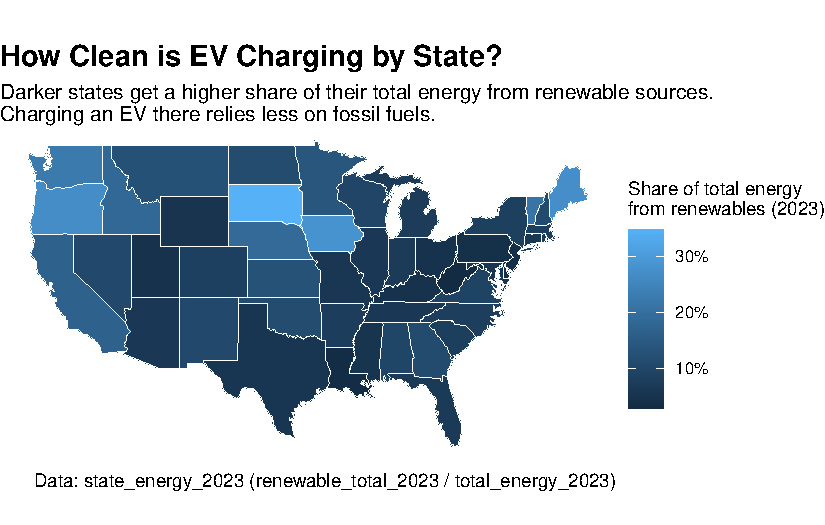
\includegraphics[keepaspectratio]{report_files/figure-pdf/unnamed-chunk-4-1.pdf}}

\subsection{Data and Methods}\label{data-and-methods}

I used three 2023 datasets: renewable energy use by state, total energy
use by state, and EV registrations by state. I cleaned the column names,
converted messy strings like ``3404 kWh'' and ``\#13047'' into numbers,
and made sure all states used the same two-letter abbreviations. I then
summed renewable energy per state and total energy per state, and merged
that with EV registrations. From this merged table, I created two new
variables. The first is renewable\_share\_2023, which is renewable
energy divided by total energy for each state. This measures how
``clean'' the electricity is in that state. The second is an EV
intensity measure that compares EV registrations to total energy use. I
also inspected the joined table (the head() of state\_energy\_2023) to
make sure it looked correct.

\subsection{Map Visualization}\label{map-visualization}

I made a choropleth map of the U.S. where each state is shaded by
renewable\_share\_2023. Darker states get more of their total energy
from renewables, which means charging an EV there is more likely to use
clean electricity. Lighter states still rely more on fossil fuels to
generate electricity. The map includes a title (``How Clean is EV
Charging by State?''), a subtitle explaining how to read the colors, and
a legend labeled as ``Share of total energy from renewables (2023).''
This map directly shows where EV charging is closest to truly
low-emission.

\subsection{Analysis}\label{analysis}

The results are not the same everywhere. States like South Dakota, Iowa,
Washington, and Oregon get a very high share of their total energy from
renewables. In those states, charging an EV is already relatively clean,
because the grid itself is clean. California is especially interesting
because it has both a fairly high renewable share and a very large
number of EVs on the road, so people there are actually charging lots of
EVs on a cleaner grid. In contrast, some states with many EVs, like
Texas and Florida, have much lower renewable shares. That means EVs
there still improve local air quality (no tailpipe exhaust), but the
electricity that charges them still often comes from fossil fuels. There
are also states with clean grids but not many EVs yet. Overall, the
takeaway is: EVs are not equally ``clean'' everywhere. Whether charging
an EV is truly low-emission depends a lot on which state you're in.




\end{document}
